%% The following is a directive for TeXShop to indicate the main file
%%!TEX root = diss.tex

\chapter{Solutions to Including Geological Maps Into \ac{MOF}}
\label{ch:GIFtools}
%
%\begin{epigraph}
%
%\end{epigraph}
%
%As Far I as I can tell This section should organized by data type as well.
%
%\section{Forms of A Priori Information}
%\label{sec:Forms of A Priori Information}
%
%\subsection{Bore Hole Data and the Use of Koenigsberger Ratios to Correct Bore Hole Susceptibility Measurements}
%\label{sec: Bore Hole Data}
%
%
%I think there is some use in describing how GIFtools does it now. Much of this work was done in \cite{williams2008geologically}. Mostly what I have done is the inclusion of lithologies and the use of Koenigsberger
%	
%\subsection{Surface Sample Data}
%\label{sec: Surface Sample Data}
%
%Again \cite{williams2008geologically} did much of this. I think the Surface Samples will be promary use in proving physical properties for the map in El Poma
%
%
%\subsection{Geological Maps}
%\label{sec: Geological Maps}

It is often the case that geological information is provided in the form of geological maps either cross section or plan view. These maps are of particular use since they provide a great deal of information over their entire surface. Cross sections can provide a great deal of information at depth and constrain as whole region often within the center of a target of interest. While plan view maps cannot provide information at depth they can constrain the entire surface of an inversion.  Constraining the surface of an inversion is of particular interest since the sensitivity of the data to the top cells is particularly high which can lead to artifacts on the surface.

Below in point form is the method I use to incorporate a pixel map

\begin{itemize}
\item load image into the GIFtools format
\begin{itemize}
	\item determine image format
	\item load image using MATLAB utilities
	\item convert image into .png style representation for faster computation
	\item using .twf file (world file) assign location and spacial resolution to the image
	\item assign a legend assigning pixel RGB values to geological unit
	\item assign topography (either number or GIFtools TOPOdata item) for visualization
\end{itemize}
\end{itemize}
\begin{figure} [h]
    \centering
    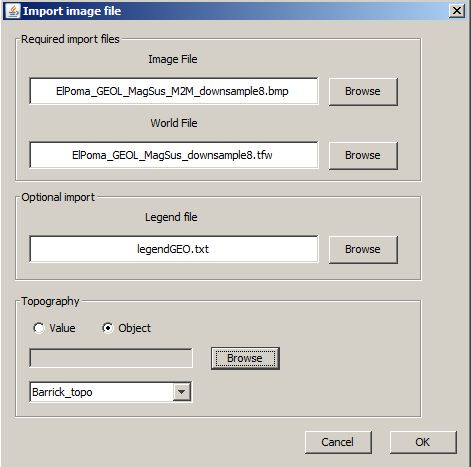
\includegraphics[width=0.5\textwidth]{images/GUI/importPlan.PNG}
    \caption{GUI for importing plan view image }
    \label{fig:importPlanGui}
\end{figure}
Storing a map as a GIFtools object allows it's use in several ways. Notably it allows the integration of the map with models and data, allowing figures overlaying the map and data or model and allowing interpretation of the data or model with direct reference to the map.

\begin{figure} [h]
    \centering
    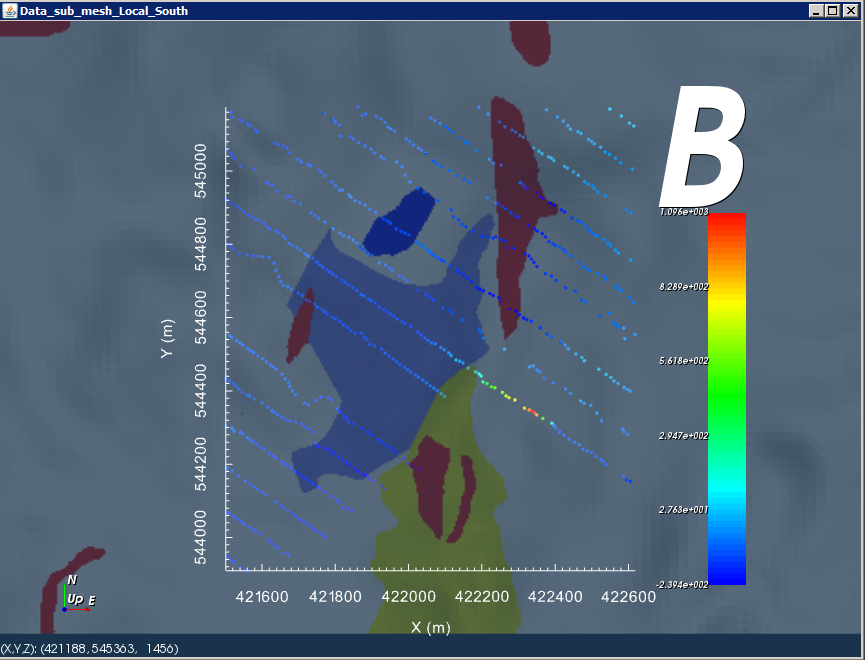
\includegraphics[width=0.5\textwidth]{images/GUI/mapData.PNG}
    \caption{Example of magnetics data being viewed with a map overlaid }
    \label{fig:mapData}
\end{figure}


Continuing on in the process of making a geological constraint
\begin{itemize}
\item find the geological value of each pixel
\begin{itemize}
	\item in the .png style format as stored in MATLAB an image consists of an ``image' field', a matrix of integers, and a ``map'' field, which maps the image matrix to RBG value triplets
	\item Each RGB triplet is compared to the legend that was provided when the image was loaded. A map field entry is considered to represent a geological unit if all three components of the RGB triplet are within a provided tolerance of any entry in the legend
	\item now that we have a relation of entries in the map field to geological units in the legend, we can assign a geological unit to each pixel in the original image simply by applying the new geological map to the image field.
\end{itemize}
\end{itemize}

now in the plan view case

\begin{itemize}
\item provide active model	
\begin{itemize}
	\item this simultaneously provides a discretized topography for the map to lay along and also a mesh (\ac{GIF} 3D tensor or OcTree) 
\end{itemize}
\item provide some form of depth information
\begin{itemize}
	\item Thickness, a certain amount of depth below topography at each point will be assigned the geological unit at each 
	\item Depth, the map will be used to assign a geological unit down to a fixed depth across the while model
	\item Surface, if you provide another surface below topography the cells between topography and the other surface will be assigned
\end{itemize}

\item crop all pixels that extend outside of the mesh or that represent the background geological unit
\begin{itemize}
	\item the cropping greatly speeds up the process and makes it require much less RAM
	\item this also means that in the event of a mistake with coordinates the process ends almost instantly since there are almost no pixels to process
\end{itemize}
\item Finally the geological model is created
\begin{itemize}
	\item We determine which cell of the mesh each pixel is in, including those cells below each pixel to account for thickness
	\item each cell is assigned a geological unit based on the mode of the geological value of each pixel
	\item the geology definition which will allow the assignment of physical properties to each geological unit
\end{itemize}
\end{itemize}

\begin{figure} [h]
    \centering
    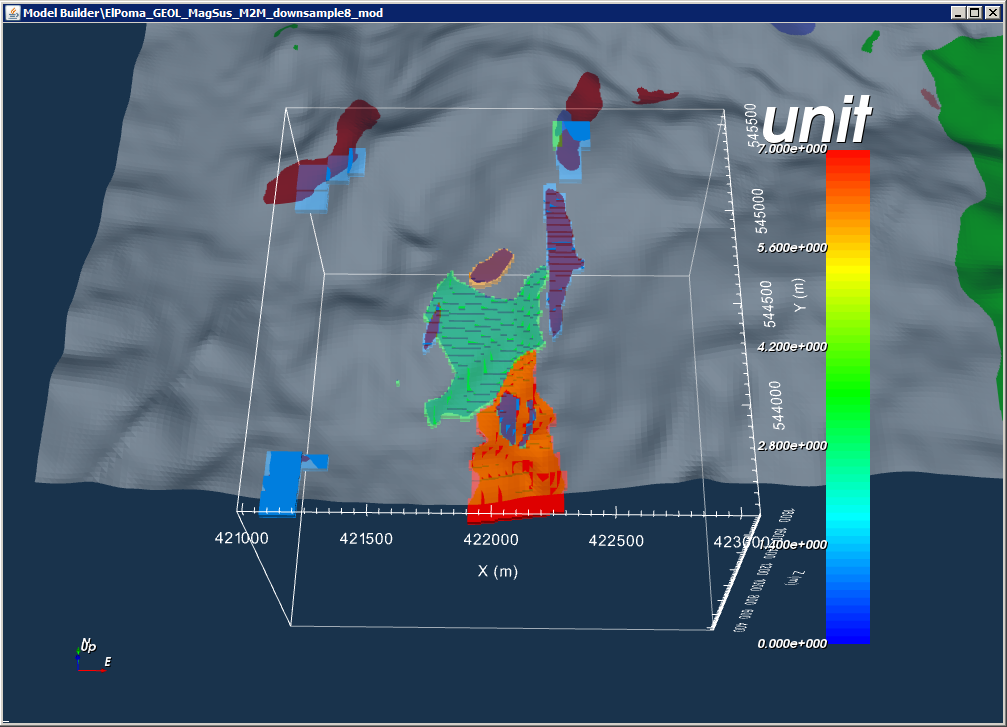
\includegraphics[width=0.5\textwidth]{images/GUI/mapModelPlan.PNG}
    \caption{Example of a geology model created from a map with the map overlaid}
    \label{fig:mapModelPlan}
\end{figure}

The cross section case follows much the same procedure with a few exceptions. An imported cross section map is shown overlaid on a 2D mesh in \autoref{fig:mapMeshCros}. Notably no parameter for the vertical extent is needed. The other notable exception is that mesh that is used is a \ac{GIF} 2D mesh. The result is shown in \autoref{fig:mapModelCross}.  After the 2D geology model is created from the cross section map it can be inserted into a 3D mesh (\ac{GIF} 3D tensor or OcTree) given a starting and ending position or a starting position and a direction.
\begin{figure} [h]
    \centering
    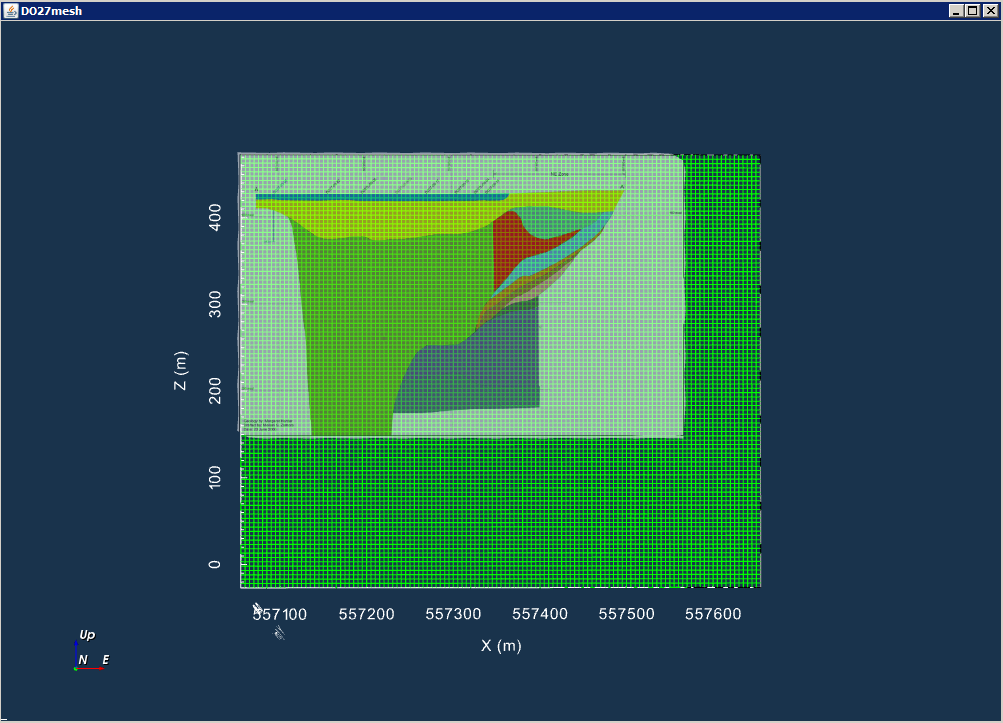
\includegraphics[width=0.5\textwidth]{images/GUI/mapMeshCross.PNG}
    \caption{Example of a 2D mesh with the map overlaid}
    \label{fig:mapMeshCross}
\end{figure}

\begin{figure} [h]
    \centering
    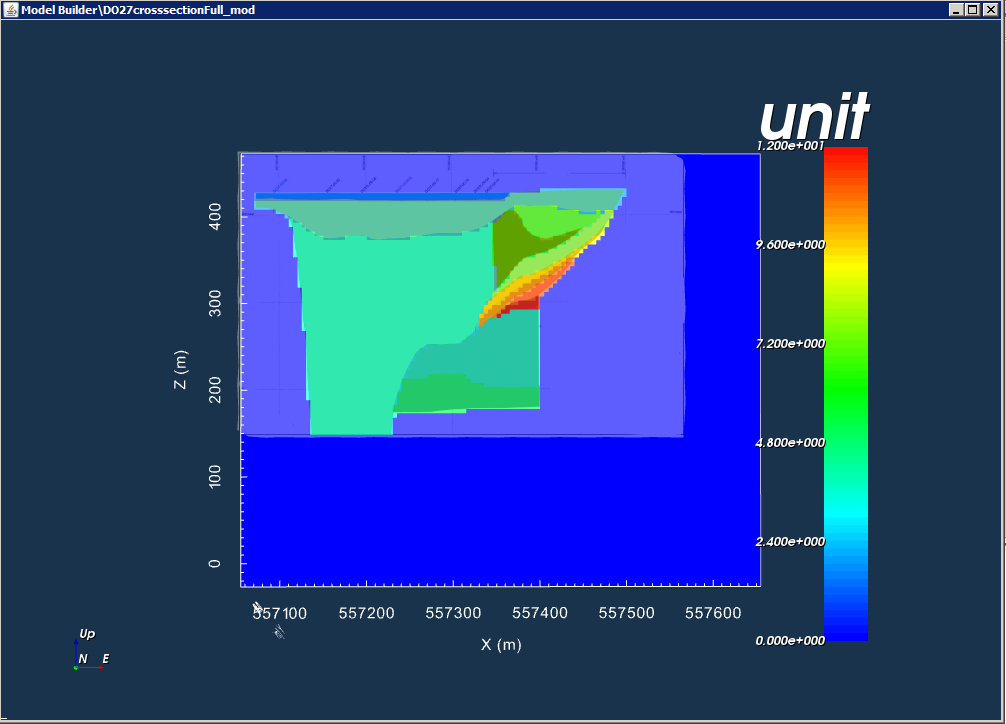
\includegraphics[width=0.5\textwidth]{images/GUI/mapModelCross.PNG}
    \caption{Example of a 2D geology model created from a cross section map with the map overlaid}
    \label{fig:mapModelCross}
\end{figure}






%\section{Using Multiple Data Types, with Clustering}
%\label{sec:Using Multiple Data Types, with Clustering}
%
%There is interesting things to discuss in the storing of multiple inversion in GIFtools, and in the use of clustering algorythms used and then ability to take geological models and make reference models and non-trivial face weighting.

\endinput

 Interestingly, the assumption that all magnetizations are in the same direction also assumes that all Koenigsberger ratios are equal.

Any text after an \endinput is ignored.
You could put scraps here or things in progress.
